\documentclass[12pt]{article}
\usepackage{xeCJK}
\usepackage{graphicx}
\usepackage{amsmath}
\usepackage{enumerate}
\usepackage{diagbox}
\usepackage{url}
\newcommand{\Zmod}{\left|Z\right|}

\begin{document}
\title{数字逻辑设计报告 \quad Music3D组}
\author{潘传宇 \quad 任一}
\maketitle

\newpage
\tableofcontents

\newpage
\section{实验目的}
本实验的最终目的是希望实现一个\textbf{能够接收音频信号,并将音乐的律动以“立体”的方式显示出来的音频可视化系统}。
其中我们使用AN831模块作为音频的输入模块,并使用光立方模块作为“立体显示”模块。
具体目标有以下几点:
\begin{enumerate}
    \item 实现音频的数字信号输入及处理;
    \item 借助FFT算法实现音频的时域信号向频域信号转换;
    \item 实现频域信号向光立方所需的灯光信号的转换;
    \item 实现灯光信号的“队列式”存储与移位;
    \item 实现灯光信号的“整合打包”与串口协议输出;
\end{enumerate}

\section{实验完成情况与任务分工}
\subsection{完成情况}
\begin{center}
    \begin{tabular}{|c|c|}
        \hline
        时间& 任务\\
        \hline
        第九、十周& 确定主题以及大致设计框架,购买外设,熟悉FPGA板使用\\
        \hline
        第十一周& 确定设计框架,开始编写音频处理部分代码,调试外设\\
        \hline
        第十二周& 完成音频输入、串口输出部分的代码编写,进一步完善设计框架\\
        \hline
        第十三周& 完成音频FFT部分的代码编写,上板调试音频部分\\
        \hline
        第十四周& 完成灯光信号处理部分的代码编写,上板进行整体调试\\
        \hline
        第十五周& 尝试多种模式设计,优化效果\\
        \hline
        第十六周& 准备课堂展示\\
        \hline
    \end{tabular}
\end{center}

\subsection{任务分工}
\begin{itemize}
    \item 潘传宇:调试板子及外设,编写灯光信号处理部分的代码,编写光立方通信协议部分的代码;
    \item 任一: 选购音频模块AN831,编写音频输入及FFT处理部分的代码,协助调试硬件;
\end{itemize}

\section{实验演示说明}
实验演示按照如下步骤进行:
\begin{enumerate}
    \item 按照引脚分配将AN831模块和光立方模块接入FPGA板;
    \item 将板子接入电源,并将程序烧写进入板子;
    \item 启动光立方,通过设置单片机工作模式进入“串口接收模式”;
    \item 烧写完成后,板子立即进入工作状态,此时通过音频线将音频接入AN831模块后,即可看到光立方上随音乐变化的显示效果;
    \item 默认模式为“舒缓模式”,按住实验板上的reset键可进入“动感模式”;
\end{enumerate}
\begin{center}
    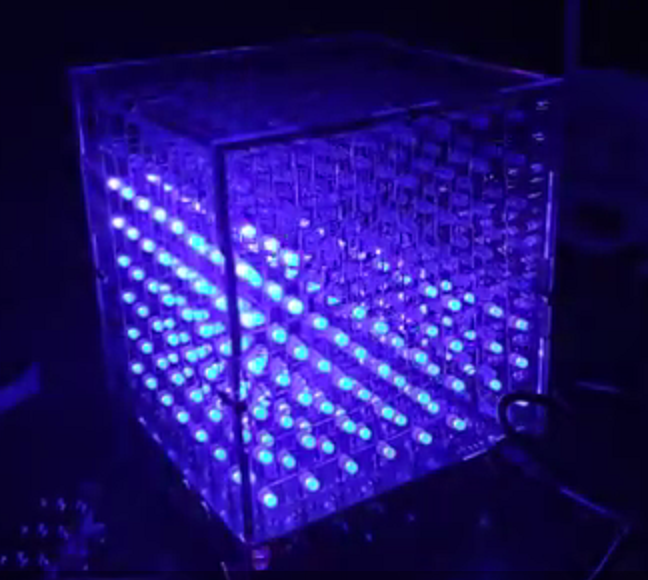
\includegraphics[scale=0.6]{pic/show1.png}
    \\\small{展示效果图}
\end{center}
展示视频链接如下:

舒缓模式:\url{https://www.bilibili.com/video/BV1na4y1Y7t9/}

动感模式:\url{https://www.bilibili.com/video/BV1rZ4y1H7Dr/}

% \newpage
\section{文件说明}
本项目文件说明如下表:\footnote{完成者中带*对应的文件,参考了\url{https://github.com/Ugon/fpga-fft-equalizer}或直接使用Altera中的PLL,并非完全独立实现。}
\begin{table}[h]
    \centering
    \resizebox{\textwidth}{!}{
    \begin{tabular}{|l|l|l|}
    \hline
    文件名                           & 功能                                       & 完成者 \\ \hline
    AN831.vhd                     & 读入AN831模块的输出,进行FFT                & 任一  \\ \hline
    audio\_processor.vhd          & 由时域数字信号做FFT得到频域数字信号                      & 任一*  \\ \hline
    dsp\_slave\_reader.vhd        & 将串行的ADCDAT以样本点为单位转为并行                    & 任一*  \\ \hline
    fft\_dif.vhd                  & 递归实现FFT                                  & 任一*  \\ \hline
    fft\_input\_deserializer.vhd  & 为FFT准备时域信号                               & 任一*  \\ \hline
    fft\_twiddle\_factors\_64.vhd & FFT计算中用到的旋转因子                            & 任一*  \\ \hline
    fft\_utils.vhd                & FFT计算中用到的函数                              & 任一*  \\ \hline
    i2c\_clk\_prescaler.vhd       & 时钟分频,由50MHz转换为100kHz                     & 任一* \\ \hline
    i2c\_master\_writer.vhd       & 配置WM8731芯片寄存器                            & 任一*  \\ \hline
    mTransmitter.vhd              & 接受频域采样信息,转化为灯光信息并存储移位与整合输出                                         & 潘传宇 \\ \hline
    mTXD.vhd                      & 并行信号转UART串口输出                                         & 潘传宇 \\ \hline
    mw8731\_controller.vhd        & 处理ADCDAT,配置WM8731芯片寄存器                & 任一*  \\ \hline
    mypll.vhd                     & 时钟分频,由100MHz转换为50MHz                     & 任一*  \\ \hline
    top.vhd                       & 顶层模块,连接音频处理和灯光信息传输模块 & 任一、潘传宇  \\ \hline
    trans\_pkg.vhd                & 定义若干新数据类型                                         & 潘传宇 \\ \hline
    \end{tabular}}
    \caption{项目文件说明}
    \end{table}
\section{总体设计}
\subsection{整体框架}
\paragraph{}本项目设计的整体框架如Figure\eqref{structure}所示。 
整个工程的输入为3.5mm的音频线,输入的是模拟信号。经过AN831模块中的WM8731芯片的模数转换,
得到24位的数字信号。数字信号输入FPGA后,由FPGA做FFT和数据的打包处理,由RX/TX串口将灯光信号
发送给光立方,光立方产生显示效果。


\begin{figure}[h]
    \centering
    \label{structure}
        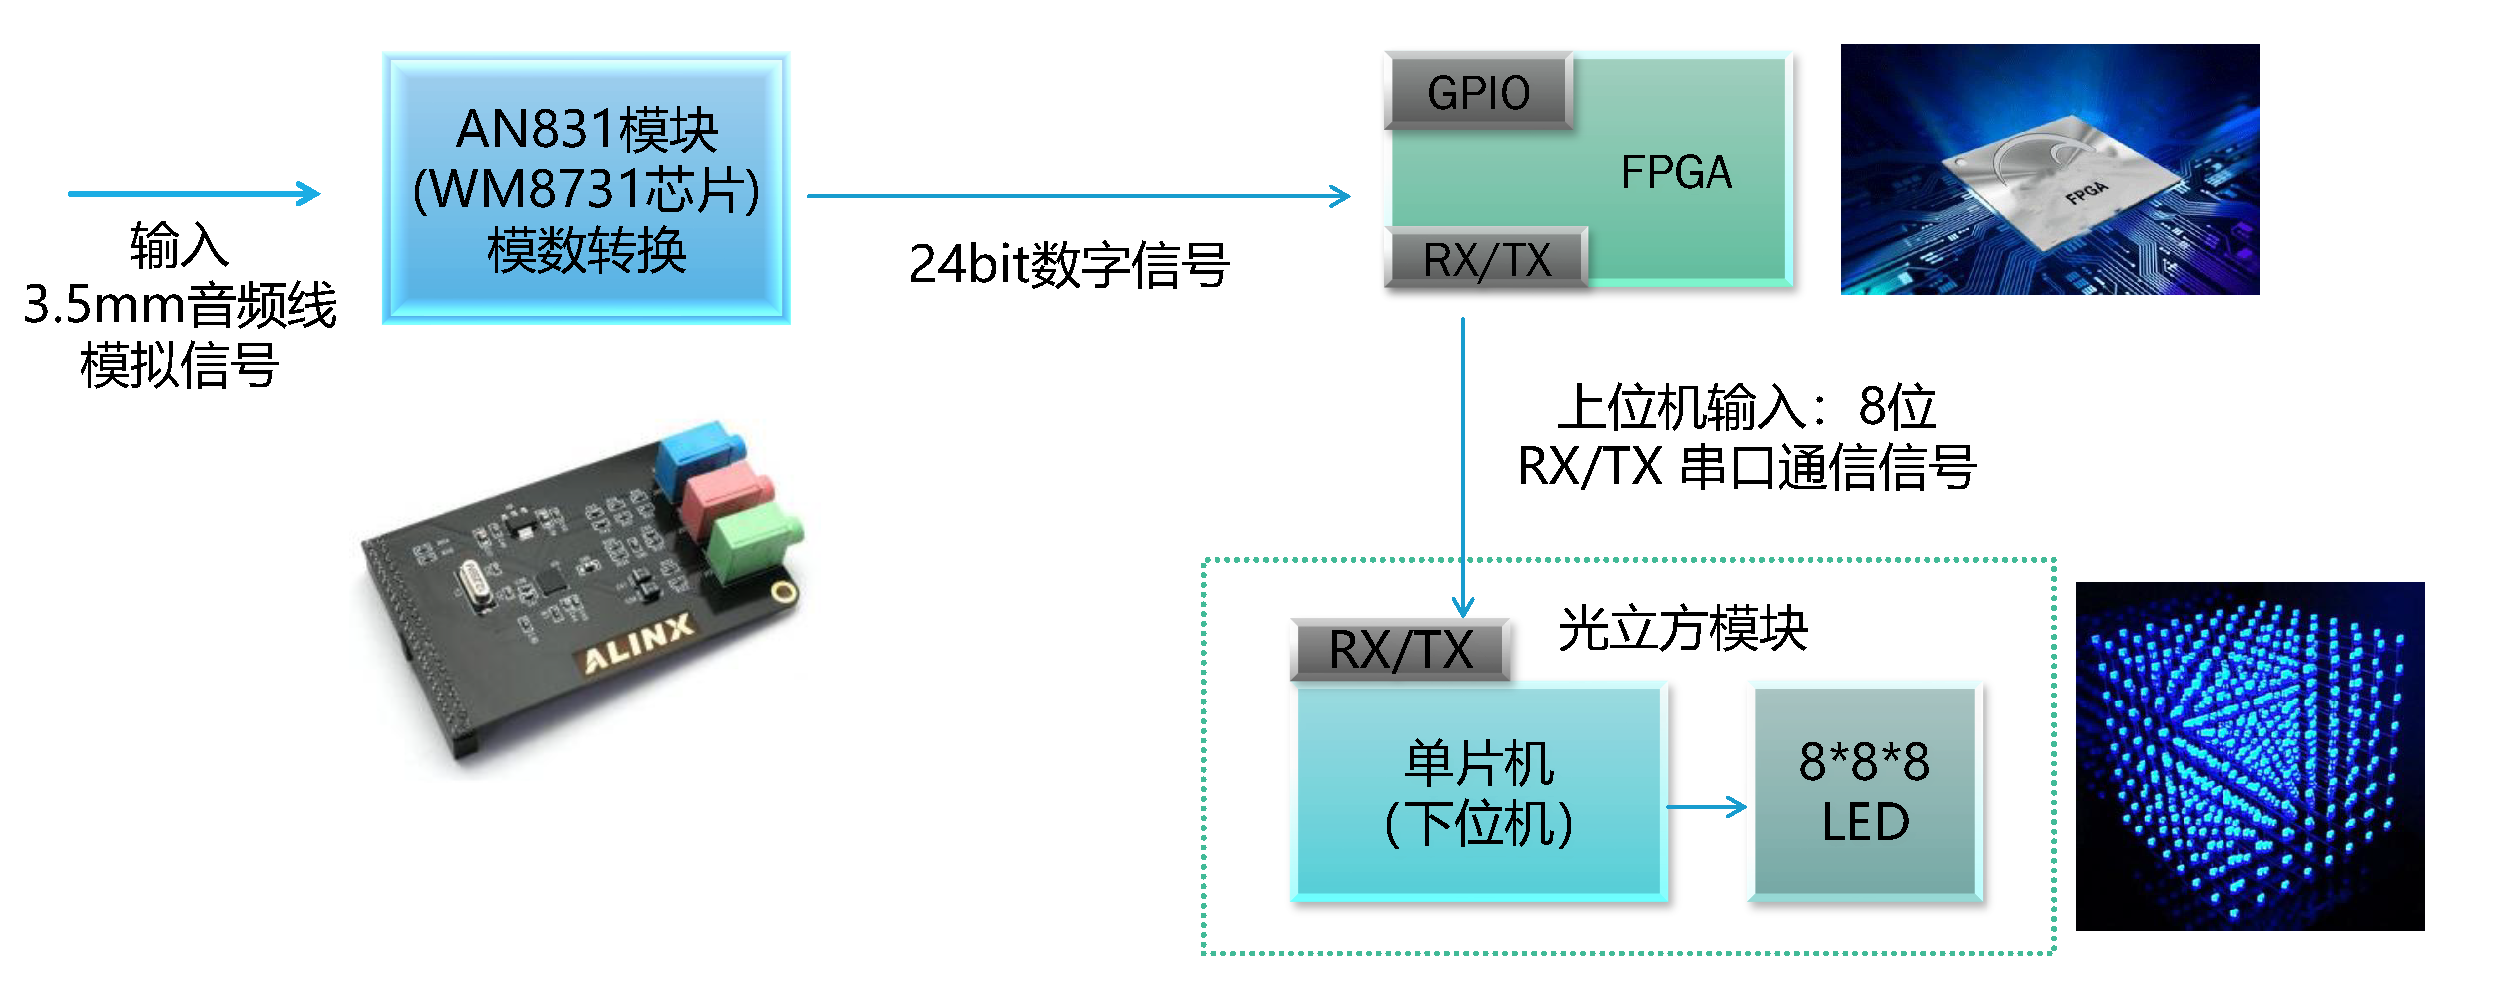
\includegraphics[width=0.8\textwidth]{./pic/structure.png}
        \caption{整体框架图}
\end{figure}

\clearpage
\subsection{FPGA设计概要}
\paragraph{}
FPGA设计概要如Figure\eqref{Design}所示。在FPGA中,我们首先接收了AN831模块输出的时域数字串行信号,并将其转为并行,
之后进行FFT,得到频域信号,由频域信号再转为灯光信息。
接着将灯光信息进行存储和整合,最后由UART串口输出给光立方。

\begin{figure}[h]
    \centering
    \label{Design}
        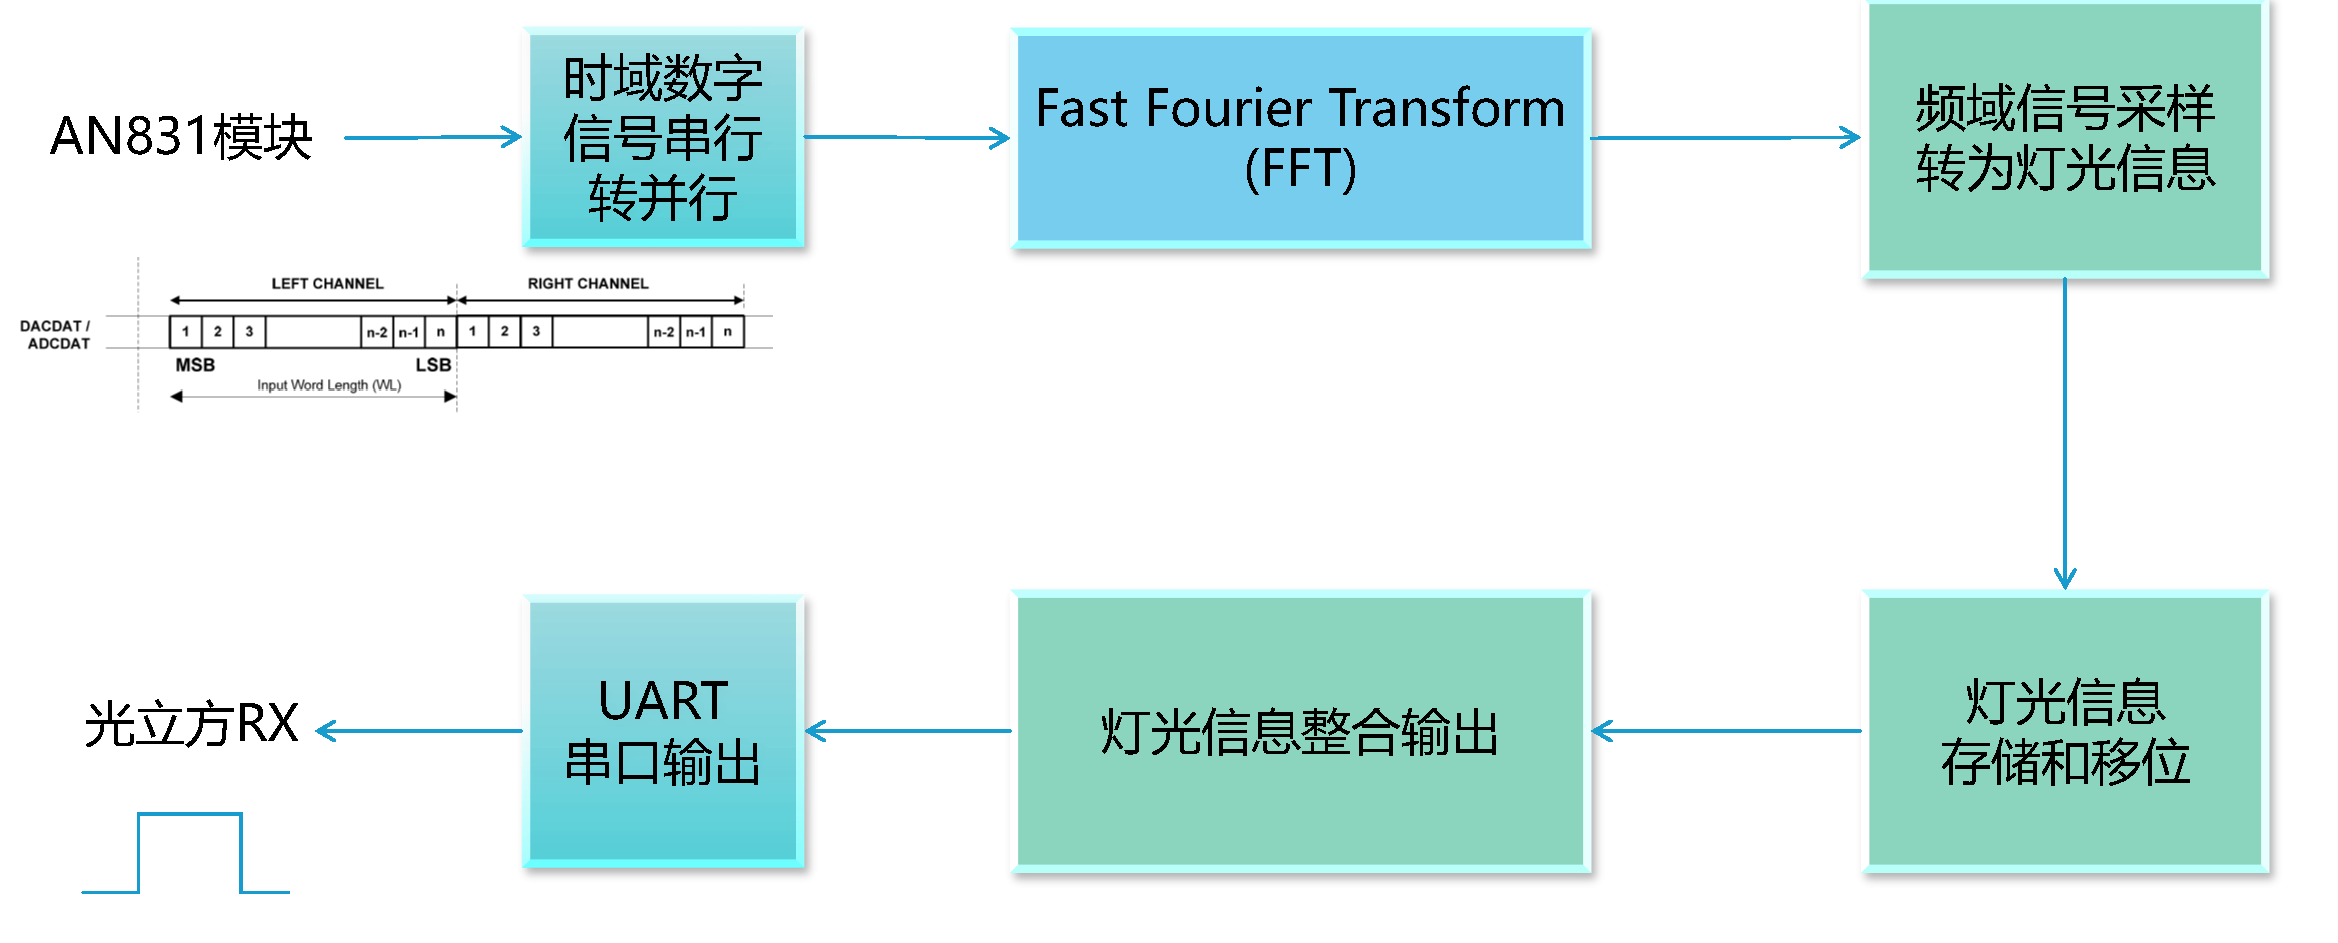
\includegraphics[width=0.8\textwidth]{./pic/Design.png}
        \caption{FPGA设计概要图}
\end{figure}

\subsection{光立方工作示意}
\paragraph{}
光立方的工作原理示意如Figure\eqref{cube}所示。
光立方是三维的显示,三个维度分别是时间、频率和强度。
随着时间的推移,光立方的显示沿着时间轴队列式逐层后移。
从频率-强度平面来看,光立方的8列分别代表8个频率分量的强度。
亮灯多的列对应的频率分量强度大,亮灯少的列对应的频率分量强度小。
同时,音量的大小也与强度有一定正相关关系,音量大则强度大,音量小则强度小。

\begin{figure}[h]
    \centering
    \label{cube}
        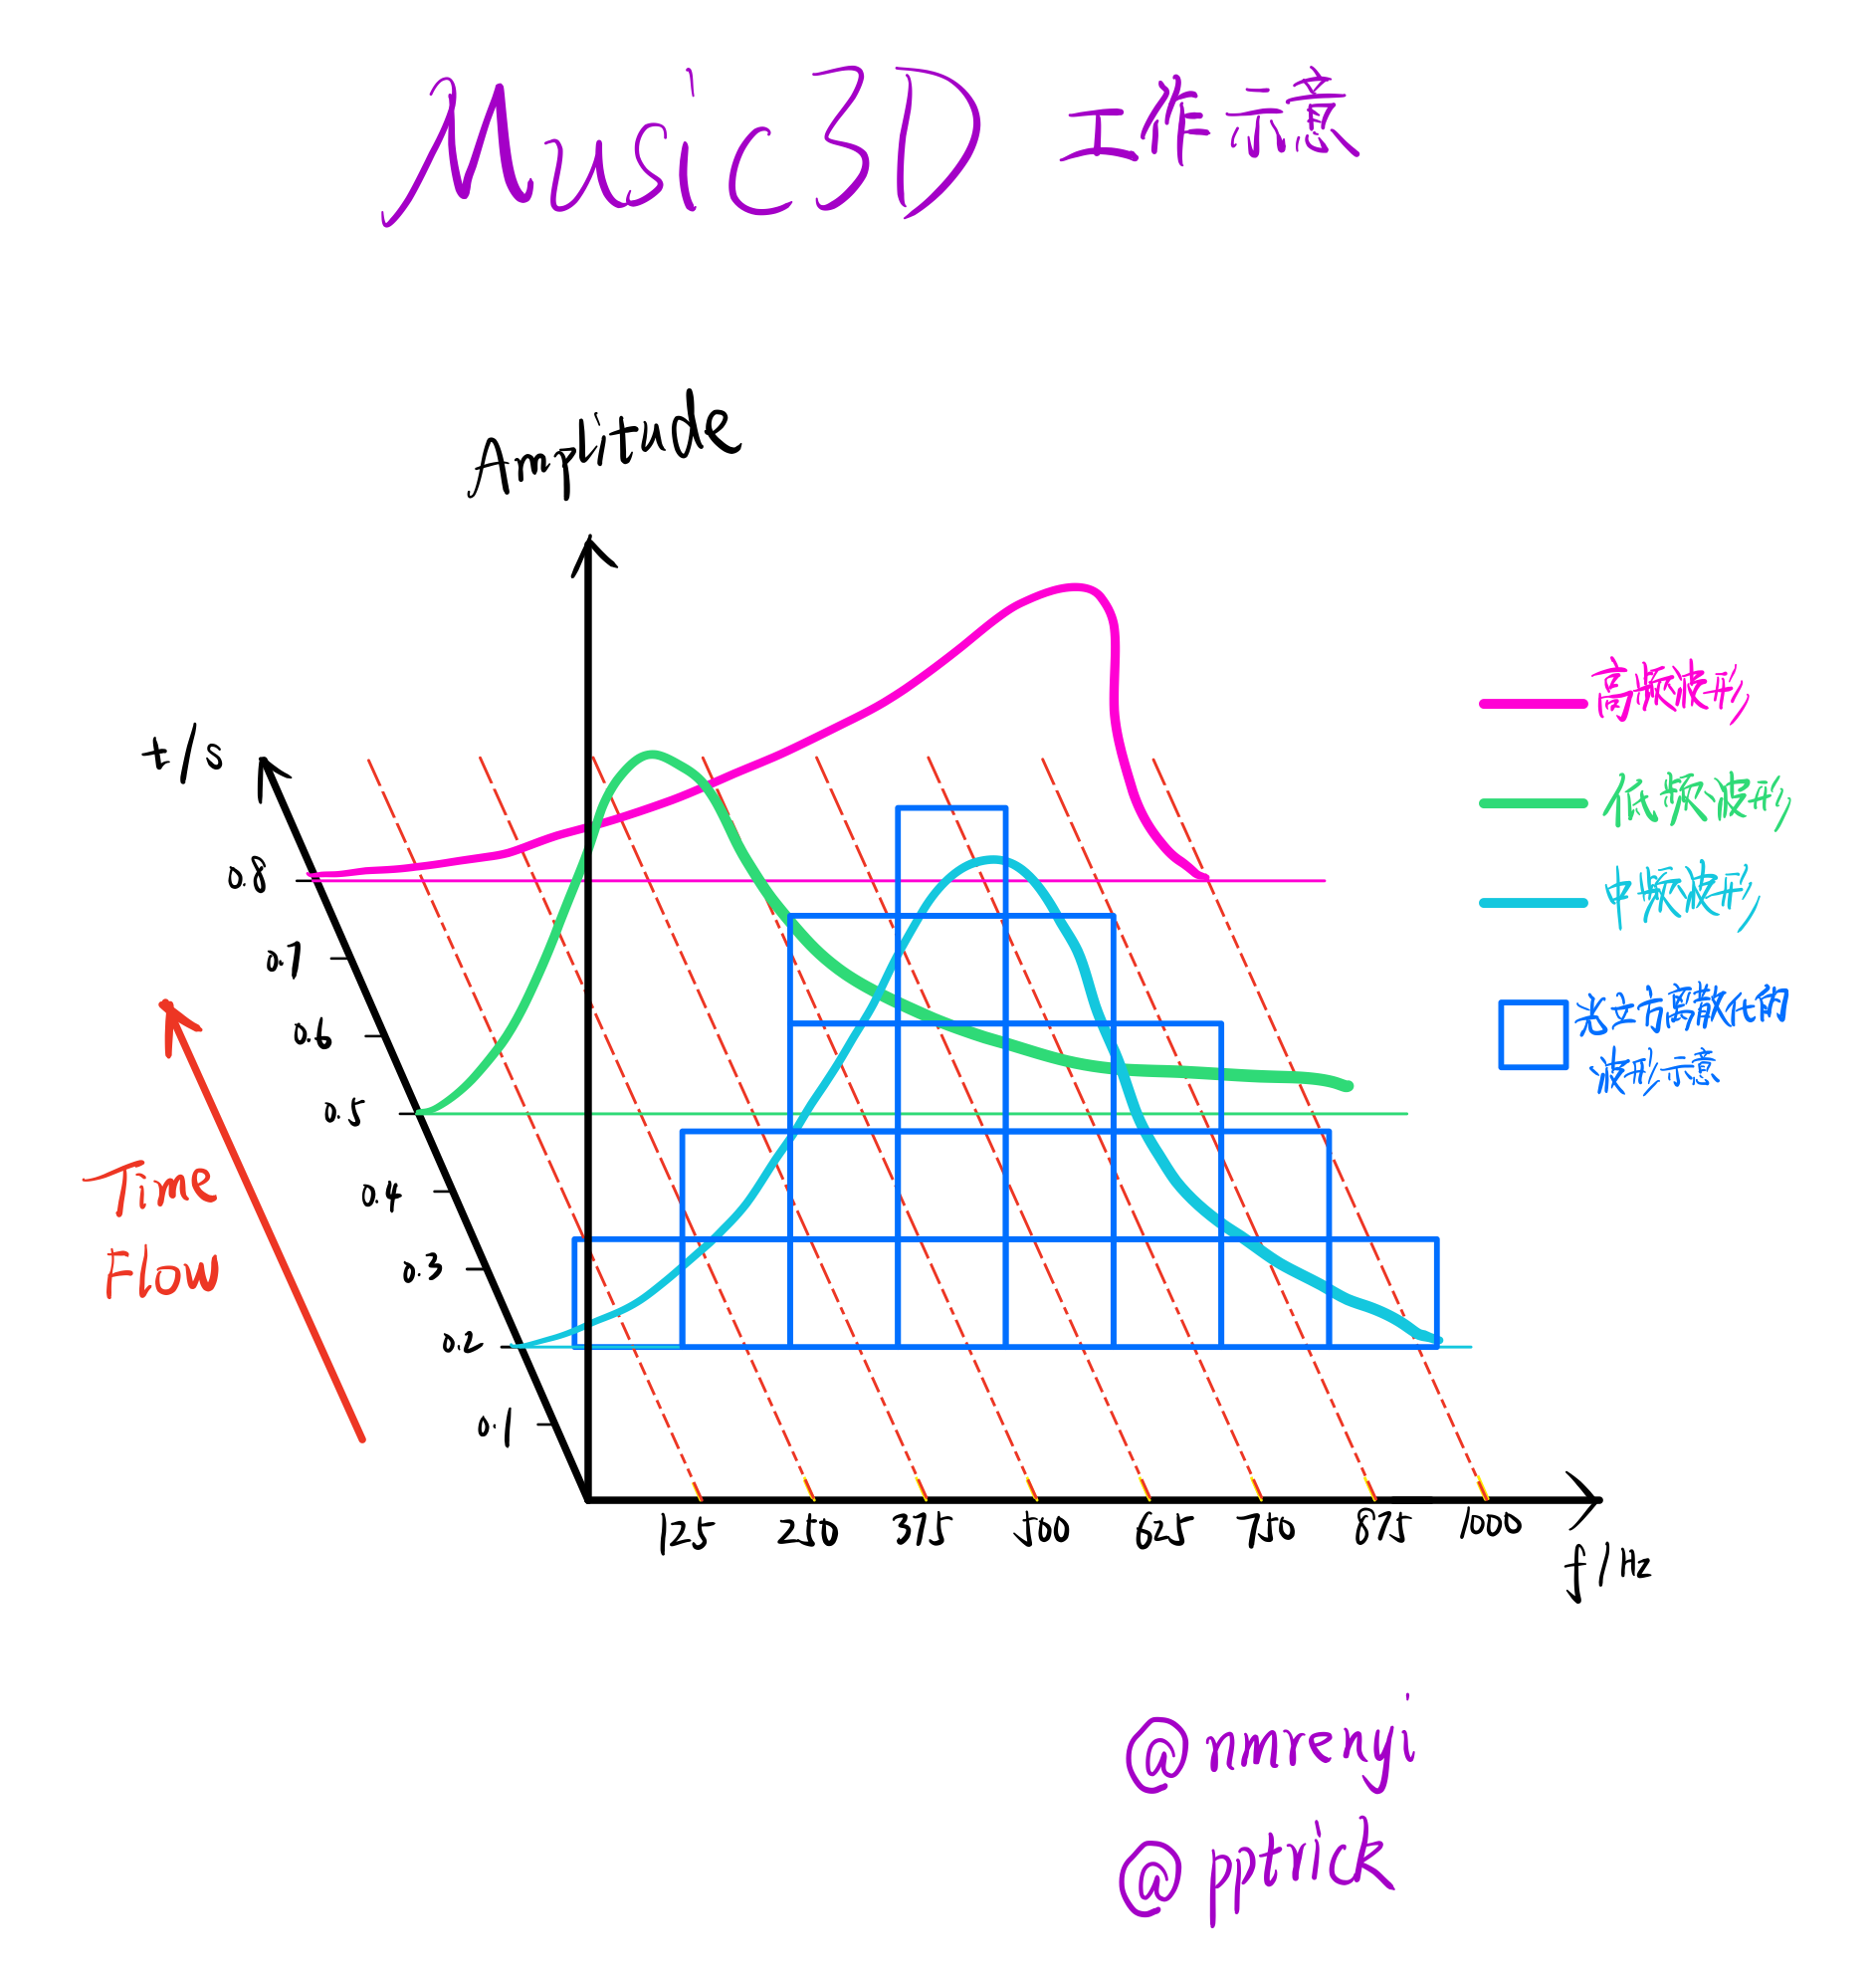
\includegraphics[width=0.74\textwidth]{./pic/ProjectWork.png}
        \caption{光立方工作原理示意图}
\end{figure}

\newpage
\section{关键技术分析}
\subsection{Fast Fourier Transformation}
\paragraph{}为了从时域信号中提取频域信息,我们需要使用快速傅里叶变换(FFT)。在本代码中,我们配置WM8731芯片的采样频率为8KHz, 进行64点的FFT,得到了125Hz, 250Hz, 375Hz, 500Hz, 625Hz, 750Hz, 875Hz, 1000Hz
这8个频率处的频谱分量,正好对应光立方每一帧的8列灯光信息。为了节约计算成本,我们在进行FFT时,通过定点数的方式,提前储存了旋转因子。

\subsection{串口协议通信}
\subsubsection{WM8731串口协议}
\paragraph{}
在本项目中,我们使用了WM8731的DSP工作模式。在该模式下,左右声道信号在BCLK和LRCLK信号的控制下,通过ADCDAT进行传输。下图为信号传输协议示意图。

\begin{figure}[h]
    \centering
    \label{dsp}
        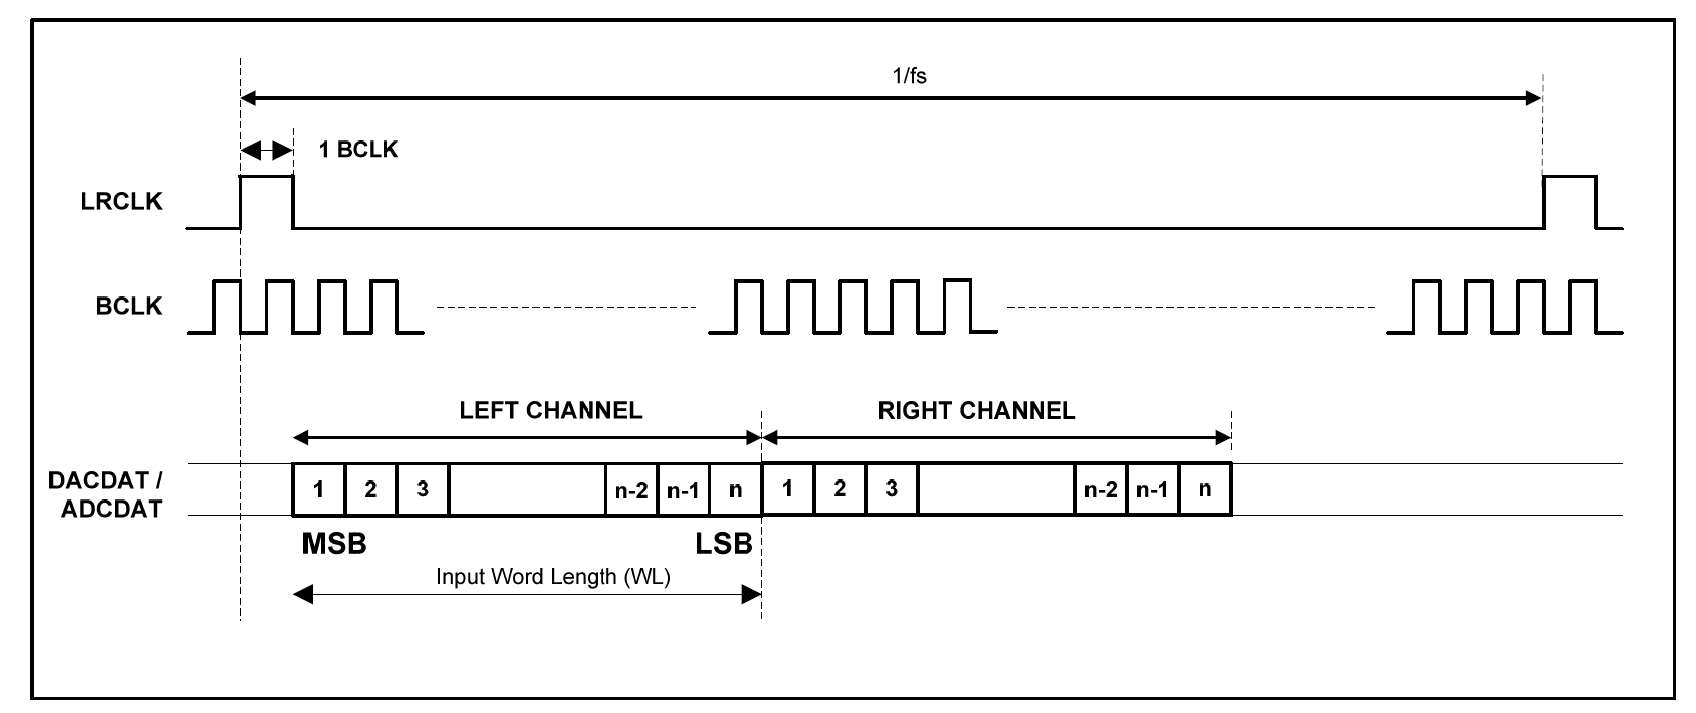
\includegraphics[width=0.74\textwidth]{./pic/dsp.png}
        \caption{DSP模式下,WM8731串口传输协议示意图}
\end{figure}

\subsubsection{光立方串口协议}
\paragraph{}通过UART串口传送串行信号,可以将设计好的灯光信息传给光立方模块上的单片机(相当于下位机),并由单片机控制灯的亮灭。
每一时刻的灯光信号由65个8位(并行)逻辑向量构成,需要将这些8位并行数据转化为串行的01输出,因此需要编写串口协议通信模块。该模块基于状态机
实现,通过不同状态表示当前输出处于起始位、数据位、校验位还是停止位,并通过计数方法使之适应相应的波特率。

\subsection{灯光信息整合输出}
\paragraph{}灯光信息采用“队列”结构存储,即每一时刻由采样模块收集频域信息并转化为灯光信息,将该灯光信息传入“队尾”,然后将“队顶”信息弹出。
\paragraph{}每次传给光立方的数据是65个8位逻辑向量,它是由1个“起始位”和64个“数据位”构成的;在传输时需要依次将这些8位逻辑向量传给“串口通信模块”。实现这一功能的难点在于与频域采样频率和串口波特率之间相适配。
此模块同样基于状态机实现,用不同状态判断当前输出处于起始位、数据位还是停止位;同时由于采样频率远小于波特率,可以通过计数方法将灯光信息输送频率调整到一个较为恰当的值。



\section{程序注释}
一些重要信号的说明如下表:
\begin{table}[h]
    \centering
    \resizebox{\textwidth}{!}{
    \begin{tabular}{|c|c|c|c|}
        \hline
        信号名& 所属实体& 数据类型& 说明\\ 
        \hline
        iCLK\_100& top& std\_logic& 100MHz时钟输入\\
        \hline
        iCLK\_11Mhz& top& std\_logic& 11.0592MHz时钟输入\\
        \hline
        Mode& top& std\_logic& 模式选择:舒缓模式、动感模式\\
        \hline
        AUD\_BCLK& top& std\_logic& 一个时钟信号,频率为$2\times SampleFrequency \times BitsPerSample$ \\
        \hline
        AUD\_ADCLRCK& top& std\_logic&控制左右声道输出的时钟信号 \\ 
        \hline
        iAUD\_ADCDAT& top& std\_logic&WM8731芯片模数转换得到的数字信号 \\ 
        \hline
        tx\_out& top& std\_logic& UART串口信号输出(给光立方)\\
        \hline
        I2C\_SDAT& top& std\_logic& I2C协议中,控制WM8731芯片寄存器的信号 \\
        \hline
        oI2C\_SCLK& top& std\_logic& I2C协议中的一个时钟信号 \\
        \hline
        out\_page& AN831& std\_logic\_vector(64)& 单帧(每一时刻)灯光信号\\
        \hline
        out\_page\_sample\_available& AN831& std\_logic& 用于指示out\_page是否可用\\
        \hline
        data\_in& mTransmitter& std\_logic\_vector(64)& 同out\_page,灯光信息输入\\
        \hline
        send\_cmd& mTransmitter& std\_logic& 同out\_page\_sample\_available,上升沿抓取灯光信息\\
        \hline

    \end{tabular}}
    \caption{重要信号说明}
\end{table}


\section{遇到问题与解决方法}
\subsection{FPGA逻辑资源不足}
\paragraph{}在最初的项目调试中,我们希望做到的是采样频率48kHz的1024点FFT。这样做存在的问题是,
由于FFT涉及到大量的乘法,导致板子的逻辑资源严重不足。

因此我们从两方面进行改进,一方面是降低FFT点数,从1024点降低到64点,使得计算复杂度降低,同时我们也降采样频率
由48kHz降低到8kHz,从而保证FFT得到的每两点之间的频率差不会过大。另一方面,我们降低了旋转因子定点数的位数,从
原项目的16bit旋转因子降低到14bit旋转因子,进一步降低了计算的复杂度。通过这两方面的改进,我们成功实现了采样频率为8kHz下,64点的FFT。

其他可能的改进思路还有降低采样深度(即bits per sample). 这样做的原理与降低旋转因子的位数相似,都能够降低FFT中乘法的资源使用。
但由于本项目使用的是WM8731的DSP模式传输数据,在DSP模式下WM8731模块仅支持24bit的采样深度,因此我们最终没有采用这种优化方案。此外,也可以
考虑从FFT的算法本身进行改进,例如利用移位代替乘除法等方法,降低硬件逻辑资源使用率。

\subsection{时序问题}
\paragraph{}在编译时,我们曾遇到Critical Warning(332148): Timing requirements not met. 这样的问题。
经过与助教讨论,我们意识到这是时序出现了问题。
经过对项目中使用的时钟加入限制后,再次编译基本解决了这个问题。

\subsection{一些硬件调试的问题}
\paragraph{}最早使用AN831模块时没有反应,且伴有发热现象,经错误检查后发现正负极接反;通常来说外设板上不会显式标注正负极,需要自己判断;一个比较好的判断方法是看焊盘,方形一般为“地”。
\paragraph{}在串口连线时,TX需与RX连接、RX需与TX连接,最早调试光立方时出错检查了很长时间。
\paragraph{}实验中还出现过AN831模块无法正常传输信号的情况,经检查发现为实验板的5V电源供电不稳定。通过重新烧录程序或者更换新的电源能够解决问题。

\section{实验总结}
\paragraph{}
这一学期的数字逻辑设计课程对我来说是一次很难忘的体验。之前我只对于底层的电路和顶层的程序设计有所了解,而对中间的硬件模块化设计知之甚少;数设课程很好地填补了这一块的知识盲区。数设不同于其他同类型课程最重要的一点,我觉得在于设计和上板调试的训练;只有真正在硬件上实际操作时,才能感受到硬件设计与软件编程不同之处。

当然我觉得能够有幸和任一这么一位靠谱的队友一起奋战数月,并且看着我们的设计成果慢慢接近预设的目标应该是最有成就感也是最值得回忆的事吧,同时也非常非常感谢老师和助教们专业且耐心的指导。要说给之后上数设同学的建议,大概是一定不要吝啬调试验证的时间,每个模块设计好之后一定要充分的调试检查,尽管有时候调试时间比设计时间还要久。不过最重要的还是keep yourself occupied and enjoy it!

\rightline{————潘传宇}

\paragraph{}
数字逻辑设计课是一门很有趣的课。前半部分的理论和后半部分的实验相辅相成。非常感谢老师和助教给予我们耐心而细致的指点,也很高兴能和潘传宇同学一起组队。能够自己选择项目内容并一步步实现,是一个富有挑战但也收获了知识和乐趣的过程。在这个过程中,我锻炼了团队协作、解决问题、寻求帮助、查找资料等各方面的能力。

谈到最后较为顺利地完成项目的经验的话,从我们组的角度来看,主要是在一开始选择难度适当的题目,并合理规划进度。在选题时我们经过充分调研最终选择了在光立方上做音频可视化任务,并与老师和助教沟通了可行性和难度。此外我们组整体进度把握较好,在13周末就达成了阶段性成果,15周周一基本达到了预期结果,剩余一周则进行了充分的调优和展示的准备,因此能够有条不紊地完成整个项目。 

\rightline{————任一}



\end{document}